\documentclass[12pt,a4paper]{article}

% ─── Page Layout ───────────────────────────────────────────────────────────────
\usepackage[a4paper, margin=0.8in, headheight=14pt]{geometry}

% ─── Fonts (XeLaTeX) ───────────────────────────────────────────────────────────
\usepackage{fontspec}
\usepackage{unicode-math}
\setmainfont{TeX Gyre Pagella}
\setmonofont[Scale=0.88]{TeX Gyre Cursor}
\setmathfont{Latin Modern Math}

% ─── Packages ──────────────────────────────────────────────────────────────────
\usepackage{xcolor}
\usepackage{colortbl}
\usepackage{titlesec}
\usepackage{enumitem}
\usepackage{tabularx}
\usepackage{booktabs}
\usepackage{array}
\usepackage{amsmath}
\usepackage{tikz}
\usetikzlibrary{shapes.geometric, arrows.meta, positioning, calc, fit, decorations.pathreplacing}
\usepackage{tcolorbox}
\tcbuselibrary{skins, breakable}
\usepackage{hyperref}
\usepackage{fancyhdr}
\usepackage{graphicx}
\usepackage{microtype}
\hyphenpenalty=10000
\exhyphenpenalty=10000
\sloppy
\usepackage{caption}
\usepackage{setspace}
\usepackage{multirow}
\usepackage{tocloft}

% ─── Q&A helper ────────────────────────────────────────────────────────────────
\newcommand{\Q}[1]{\textbf{#1}\par\noindent\ignorespaces}

% ─── Colour Palette ────────────────────────────────────────────────────────────
\definecolor{myred}{RGB}{196,30,58}
\definecolor{mydark}{RGB}{30,30,50}
\definecolor{mygreen}{RGB}{14,120,80}
\definecolor{myteal}{RGB}{0,130,140}
\definecolor{myamber}{RGB}{180,100,0}
\definecolor{mypurple}{RGB}{100,30,160}
\definecolor{mygray}{RGB}{246,247,249}
\definecolor{mgframe}{RGB}{180,185,200}
\definecolor{watermark}{RGB}{145,150,170}
\definecolor{hdrred}{RGB}{250,232,235}
\definecolor{hdrgreen}{RGB}{220,244,233}
\definecolor{hdrteal}{RGB}{220,242,244}
\definecolor{hdramber}{RGB}{253,242,215}
\definecolor{hdrpurple}{RGB}{238,228,255}
\definecolor{hdrgray}{RGB}{238,240,245}
\definecolor{rowalt}{RGB}{250,251,253}

% ─── Section Formatting ────────────────────────────────────────────────────────
\titleformat{\section}
  {\large\bfseries\color{myred}}{\thesection.}{0.5em}{}
  [\vspace{1pt}{\color{myred}\rule{\linewidth}{0.8pt}}]
\titleformat{\subsection}
  {\normalsize\bfseries\color{myteal}}{\thesubsection}{0.5em}{}
\titlespacing*{\section}{0pt}{18pt}{7pt}
\titlespacing*{\subsection}{0pt}{11pt}{4pt}

% ─── Paragraph ─────────────────────────────────────────────────────────────────
\setlength{\parindent}{0pt}
\setlength{\parskip}{4pt}

% ─── TOC Styling ───────────────────────────────────────────────────────────────
\renewcommand{\cfttoctitlefont}{\large\bfseries\color{myred}}
\renewcommand{\cftaftertoctitle}{\par\noindent{\color{myred}\rule{\linewidth}{0.8pt}}}
\setlength{\cftbeforetoctitleskip}{0pt}
\setlength{\cftaftertoctitleskip}{6pt}
\renewcommand{\cftsecfont}{\normalsize\bfseries\color{mydark}}
\renewcommand{\cftsecpagefont}{\normalsize\bfseries\color{mydark}}
\renewcommand{\cftsecleader}{\cftdotfill{\cftdotsep}}
\setlength{\cftbeforesecskip}{7pt}
\renewcommand{\cftsubsecfont}{\small\color{mydark}}
\renewcommand{\cftsubsecpagefont}{\small\color{mydark}}
\setlength{\cftbeforesubsecskip}{3pt}
\setlength{\cftsubsecindent}{1.4em}

% ─── Table helpers ─────────────────────────────────────────────────────────────
\renewcommand{\arraystretch}{1.45}
\setlength{\tabcolsep}{6pt}
\arrayrulecolor{mydark}
\newcolumntype{B}[1]{>{\small\bfseries\raggedright\arraybackslash}m{#1}}
\newcolumntype{Y}{>{\small\raggedright\arraybackslash}X}
\renewcommand{\tabularxcolumn}[1]{m{#1}}

% ─── Header / Footer ───────────────────────────────────────────────────────────
\pagestyle{fancy}
\fancyhf{}
\fancyhead[L]{\small\color{myred}\textbf{EC301}\;\color{mydark}--- Electronic Devices}
\fancyhead[R]{\small\color{myteal}\textbf{Module 1 Notes}}
\fancyfoot[C]{\small\color{mydark}\thepage}
\fancyfoot[R]{\small\color{watermark}\textit{\copyright\ Biraj}}
\renewcommand{\headrulewidth}{0.5pt}
\renewcommand{\footrulewidth}{0.3pt}

% ─── Hyperref ──────────────────────────────────────────────────────────────────
\hypersetup{
  colorlinks=true, linkcolor=myteal, urlcolor=myteal,
  pdfauthor={Biraj Sarkar (CGEC)},
  pdftitle={EC301 --- Module 1 Notes: Energy Bands and Current Carriers}
}

% ─── tcolorbox styles ──────────────────────────────────────────────────────────
\tcbset{
  tikzbox/.style={
    colback=mygray, colframe=mgframe, boxrule=0.6pt, arc=4pt,
    left=8pt, right=8pt, top=6pt, bottom=6pt,
    colbacktitle=mgframe, coltitle=mydark,
    fonttitle=\small\bfseries
  },
  defbox/.style={
    colback=hdrgreen, colframe=mygreen, boxrule=0.8pt, arc=4pt,
    left=9pt, right=9pt, top=6pt, bottom=6pt,
    colbacktitle=mygreen, coltitle=white,
    fonttitle=\small\bfseries
  },
  formulabox/.style={
    colback=hdrteal, colframe=myteal, boxrule=0.8pt, arc=4pt,
    left=9pt, right=9pt, top=7pt, bottom=7pt,
    colbacktitle=myteal, coltitle=white,
    fonttitle=\small\bfseries
  },
  examplebox/.style={
    colback=hdramber, colframe=myamber, boxrule=0.8pt, arc=4pt,
    left=9pt, right=9pt, top=6pt, bottom=6pt,
    colbacktitle=myamber, coltitle=white,
    fonttitle=\small\bfseries
  },
  masonbox/.style={
    colback=hdrpurple, colframe=mypurple, boxrule=0.8pt, arc=4pt,
    left=9pt, right=9pt, top=6pt, bottom=6pt,
    colbacktitle=mypurple, coltitle=white,
    fonttitle=\small\bfseries
  },
  exambox/.style={
    colback=hdrpurple, colframe=mypurple, boxrule=1pt, arc=5pt,
    left=10pt, right=10pt, top=8pt, bottom=8pt,
    colbacktitle=mypurple, coltitle=white,
    fonttitle=\bfseries,
    breakable, title after break={\textbf{Frequently Asked / Viva Questions (contd.)}}}
}
\tcbset{breakable}

% ─── TikZ styles ───────────────────────────────────────────────────────────────
\tikzset{
  block/.style={rectangle, draw=myteal, fill=hdrteal,
    text width=2.4cm, align=center, minimum height=0.95cm,
    font=\small, rounded corners=3pt, line width=0.7pt},
  redblock/.style={rectangle, draw=myred, fill=hdrred,
    text width=2.4cm, align=center, minimum height=0.95cm,
    font=\small, rounded corners=3pt, line width=0.7pt},
  greenblock/.style={rectangle, draw=mygreen, fill=hdrgreen,
    text width=2.4cm, align=center, minimum height=0.95cm,
    font=\small, rounded corners=3pt, line width=0.7pt},
  amberblock/.style={rectangle, draw=myamber, fill=hdramber,
    text width=2.4cm, align=center, minimum height=0.95cm,
    font=\small, rounded corners=3pt, line width=0.7pt},
  purpblock/.style={rectangle, draw=mypurple, fill=hdrpurple,
    text width=2.4cm, align=center, minimum height=0.95cm,
    font=\small, rounded corners=3pt, line width=0.7pt},
  arrow/.style={-Stealth, thick, color=mydark},
  redarrow/.style={-Stealth, thick, color=myred},
  line/.style={thick, color=mydark}
}

% ═══════════════════════════════════════════════════════════════════════════════
\begin{document}
% ═══════════════════════════════════════════════════════════════════════════════

\begin{center}
  {\LARGE\bfseries\color{myred} EC301 --- Electronic Devices}\\[5pt]
  {\normalsize\color{mydark} Semester III \quad$\bullet$\quad 3L:0T:0P \quad$\bullet$\quad 3 Credits}\\[3pt]
  {\normalsize\color{myteal}\textbf{Module 1 Exam Notes: Energy Bands \& Current Carriers in Semiconductors}}\\[3pt]
  {\small\color{mydark} CGEC \;$|$\; B.Tech ECE (2023--27) \;$|$\; \textit{Biraj Sarkar}}
\end{center}
\vspace{2pt}
\noindent{\color{myred}\rule{\linewidth}{1.5pt}}
\vspace{2pt}

\hypersetup{linkcolor=mydark}
\tableofcontents
\hypersetup{linkcolor=myteal}
\newpage

% ===============================================================================
\section{Bonding Forces in Solids and Crystal Lattices}
% ===============================================================================

Electronic devices rely on the controlled movement of charge carriers through semiconductor crystalline lattices. The electrical, thermal, and optical properties of solids depend directly on the binding forces that hold their constituent atoms together.

\subsection{Types of Bonding Forces in Solids}
Atoms aggregate into solids to minimize their total potential energy by achieving filled outer electronic shells. The primary interatomic bonding forces are:

\begin{itemize}[leftmargin=*, itemsep=3pt]
  \item \textbf{Ionic Bonding:} Formed by electrostatic attraction between positively charged cations and negatively charged anions following complete electron transfer (e.g., $\text{NaCl}$). Solids exhibit high melting points and electrical insulating behavior at low temperatures.
  \item \textbf{Covalent Bonding:} Formed by sharing valence electrons between adjacent atoms to achieve a stable octet (e.g., Silicon, Germanium, Diamond). Characterized by strong directional bonds, high hardness, and semiconductor behavior.
  \item \textbf{Metallic Bonding:} Positive ion cores are immersed in a delocalized cloud or ``sea'' of free electrons. The non-directional electrostatic attraction yields high electrical and thermal conductivity.
  \item \textbf{Van der Waals (Secondary) Bonding:} Weak dipole-dipole attractions arising from temporary fluctuations in electron charge distribution (e.g., solid noble gases, graphite interlayer bonding).
\end{itemize}

\subsection{Covalent Bonding in Silicon and Germanium}
Silicon ($Z=14$) has the electronic configuration $1s^2\,2s^2\,2p^6\,3s^2\,3p^2$, and Germanium ($Z=32$) has $[\text{Ar}]\,3d^{10}\,4s^2\,4p^2$. Both are tetravalent (Group IV) with four valence electrons:

\begin{itemize}[leftmargin=*, itemsep=3pt]
  \item In a crystalline lattice, each atom forms four covalent bonds with its four nearest neighbors oriented toward the corners of a regular tetrahedron (diamond cubic lattice, coordination number $4$).
  \item At absolute zero ($T = 0\,\text{K}$), all valence electrons are locked securely in covalent bonds. No free electrons exist, and the semiconductor behaves as a perfect insulator.
  \item At room temperature ($T = 300\,\text{K}$), thermal agitation ($k T \approx 0.0259\,\text{eV}$) breaks a small fraction of covalent bonds. An electron breaks free into the conduction band, leaving behind a vacancy or ``hole'' with effective positive charge $+q$.
\end{itemize}

\begin{tcolorbox}[tikzbox, title={Covalent Bond Structure and Thermal Generation of Electron-Hole Pair}]
\centering
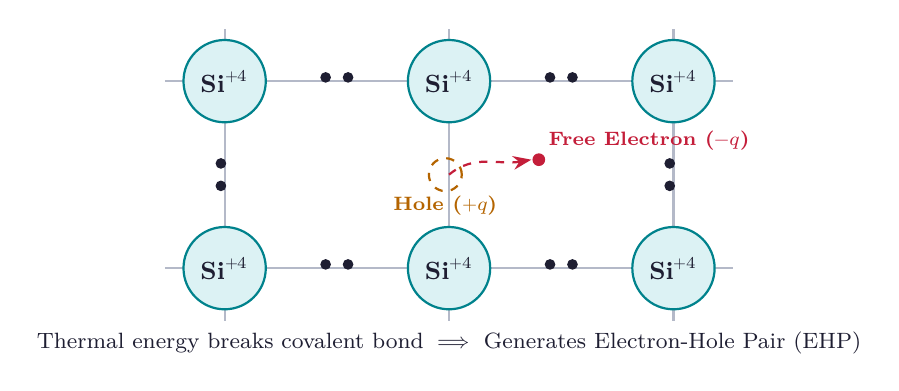
\begin{tikzpicture}[scale=0.95]
  % Define atom coordinates (3x3 grid)
  \foreach \x in {0, 3, 6} {
    \foreach \y in {0, 2.5} {
      \draw[thick, color=mgframe] (\x-0.8, \y) -- (\x+0.8, \y);
      \draw[thick, color=mgframe] (\x, \y-0.7) -- (\x, \y+0.7);
    }
  }
  % Connecting bond lines between atoms
  \draw[thick, color=mgframe] (0.8, 2.5) -- (2.2, 2.5);
  \draw[thick, color=mgframe] (3.8, 2.5) -- (5.2, 2.5);
  \draw[thick, color=mgframe] (0.8, 0) -- (2.2, 0);
  \draw[thick, color=mgframe] (3.8, 0) -- (5.2, 0);
  \draw[thick, color=mgframe] (0, 0.7) -- (0, 1.8);
  \draw[thick, color=mgframe] (3, 0.7) -- (3, 1.8);
  \draw[thick, color=mgframe] (6, 0.7) -- (6, 1.8);

  % Atoms
  \foreach \x in {0, 3, 6} {
    \foreach \y in {0, 2.5} {
      \filldraw[fill=hdrteal, draw=myteal, thick] (\x, \y) circle (0.55) node[font=\small\bfseries\color{mydark}] {$\text{Si}^{+4}$};
    }
  }

  % Valence electron dots (bonded pairs)
  \foreach \x in {1.5, 4.5} {
    \filldraw[color=mydark] (\x-0.15, 2.55) circle (1.8pt);
    \filldraw[color=mydark] (\x+0.15, 2.55) circle (1.8pt);
    \filldraw[color=mydark] (\x-0.15, 0.05) circle (1.8pt);
    \filldraw[color=mydark] (\x+0.15, 0.05) circle (1.8pt);
  }
  \foreach \y in {1.25} {
    \filldraw[color=mydark] (-0.05, \y-0.15) circle (1.8pt);
    \filldraw[color=mydark] (-0.05, \y+0.15) circle (1.8pt);
    \filldraw[color=mydark] (5.95, \y-0.15) circle (1.8pt);
    \filldraw[color=mydark] (5.95, \y+0.15) circle (1.8pt);
  }

  % Broken bond at center vertical bridge
  \draw[dashed, thick, color=myamber] (2.95, 1.25) circle (0.22) node[below=4pt, font=\scriptsize\bfseries\color{myamber}] {Hole ($+q$)};
  \filldraw[color=myred] (4.2, 1.45) circle (2.2pt) node[above right, font=\scriptsize\bfseries\color{myred}] {Free Electron ($-q$)};
  \draw[-Stealth, thick, dashed, color=myred] (3.0, 1.25) to[out=40, in=190] (4.1, 1.45);
  \node[font=\footnotesize\color{mydark}, align=center] at (3, -1.0) {Thermal energy breaks covalent bond $\implies$ Generates Electron-Hole Pair (EHP)};
\end{tikzpicture}
\end{tcolorbox}

\subsection{The Concept of Holes and Hole Conduction}
A \textbf{hole} is a conceptual quasiparticle representing an unoccupied quantum electronic state (vacancy) in an otherwise nearly filled valence band.

\begin{tcolorbox}[defbox, title={\textbf{Physics and Fundamental Properties of Holes}}]
\begin{itemize}[leftmargin=*, itemsep=3pt]
  \item \textbf{Effective Positive Charge ($+q$):} The absence of an electron (charge $-q$) from a neutral atom vacancy within a crystal lattice results in a net local positive charge of $+q = +1.602 \times 10^{-19}\,\text{C}$.
  \item \textbf{Mechanism of Hole Conduction:} When an electric field $\vec{\mathcal{E}}$ is applied across a semiconductor, an electron from an adjacent covalent bond hops into the vacancy in the direction opposite to $\vec{\mathcal{E}}$. This creates a new vacancy at the adjacent site. Macroscopically, this sequential valence electron hopping appears as the directed physical motion of a \textbf{positive charge carrier} (hole) traveling in the direction of the applied electric field $\vec{\mathcal{E}}$.
  \item \textbf{Positive Effective Mass ($m_h^*$):} Near the top of the valence band, the $E\text{-}k$ energy-momentum dispersion has downward curvature ($\frac{d^2 E}{dk^2} < 0$). An electron missing from a negative-curvature state behaves dynamically under external forces as a particle with a \textbf{positive effective mass}:
  \begin{equation}
    m_h^* = -\frac{\hbar^2}{\left(\frac{d^2 E}{dk^2}\right)_{\text{VB max}}} > 0
  \end{equation}
  \item \textbf{Hole Mobility Comparison ($\mu_p < \mu_n$):} Hole transport requires overcoming local covalent bonding potentials and hopping across tightly bound valence orbitals, experiencing higher acoustic phonon scattering. Consequently, hole mobility is always substantially lower than conduction-band electron mobility (in Silicon at $300\,\text{K}$, $\mu_n \approx 1350\,\text{cm}^2/\text{V}\cdot\text{s}$ while $\mu_p \approx 480\,\text{cm}^2/\text{V}\cdot\text{s}$).
\end{itemize}
\end{tcolorbox}

% ===============================================================================
\section{Energy Band Theory in Crystals}
% ===============================================================================

\subsection{Formation of Energy Bands}
In an isolated atom, electrons occupy sharp, discrete quantum energy levels ($1s, 2s, 2p, 3s, 3p, \dots$) governed by the Schr\"{o}dinger equation. When $N$ atoms are brought together to form a crystal lattice:

\begin{enumerate}[label=\arabic*., leftmargin=*]
  \item As interatomic spacing decreases, the wavefunctions of outermost valence electrons begin to overlap.
  \item By the \textbf{Pauli Exclusion Principle}, no two electrons in the interacting system can occupy the exact same quantum state.
  \item Each discrete atomic energy level splits into $N$ distinct, extremely closely spaced sub-levels. Because $N \sim 10^{22}\,\text{cm}^{-3}$ in a typical solid, these split levels merge into continuous \textbf{energy bands}.
  \item The energy gaps between allowed bands where no valid electron quantum states can exist are called \textbf{forbidden energy gaps} or \textbf{bandgaps} ($E_g$).
\end{enumerate}

\begin{tcolorbox}[defbox, title={\textbf{Energy Band Definitions}}]
\begin{itemize}[leftmargin=*, itemsep=2pt, topsep=0pt]
  \item \textbf{Valence Band (VB):} The highest occupied energy band formed by valence electrons. At $0\,\text{K}$, it is completely filled.
  \item \textbf{Conduction Band (CB):} The lowest unoccupied or partially filled energy band where free electrons participate in electrical conduction.
  \item \textbf{Forbidden Bandgap ($E_g$):} The energy difference between the conduction band minimum ($E_c$) and valence band maximum ($E_v$): $E_g = E_c - E_v$.
\end{itemize}
\end{tcolorbox}

\subsection{Direct vs. Indirect Bandgap Semiconductors}
The relationship between electron energy $E$ and crystal wavevector (momentum) $k$ is given by the $E$-$k$ dispersion diagram:

\begin{itemize}[leftmargin=*, itemsep=3.5pt]
  \item \textbf{Direct Bandgap Semiconductor:} The conduction band minimum and valence band maximum occur at the \textbf{same wavevector} ($k = 0$). An electron recombining with a hole across $E_g$ releases energy directly as a photon ($\Delta k = 0$):
  \begin{equation}
    E_g = h\nu = \frac{hc}{\lambda}
  \end{equation}
  \textbf{Examples:} Gallium Arsenide ($\text{GaAs}$, $E_g = 1.42\,\text{eV}$), Indium Phosphide ($\text{InP}$). Used in LEDs, laser diodes, and photodetectors.
  \item \textbf{Indirect Bandgap Semiconductor:} The conduction band minimum occurs at a \textbf{different wavevector} ($k \neq 0$) than the valence band maximum ($k = 0$). Recombination requires both an energy change and a crystal momentum change, necessitating the emission or absorption of a lattice vibration or \textbf{phonon}:
  \begin{equation}
    \Delta E = h\nu \pm E_{\text{phonon}}, \quad \Delta k = k_{\text{phonon}}
  \end{equation}
  Because a three-particle interaction (electron, hole, phonon) has low transition probability, nonradiative recombination dominates.
  \textbf{Examples:} Silicon ($\text{Si}$, $E_g = 1.12\,\text{eV}$), Germanium ($\text{Ge}$, $E_g = 0.66\,\text{eV}$). Unsuitable for efficient light emitters.
\end{itemize}

\begin{tcolorbox}[tikzbox, title={Direct vs. Indirect Bandgap Transitions ($E$-$k$ Diagrams)}]
\centering
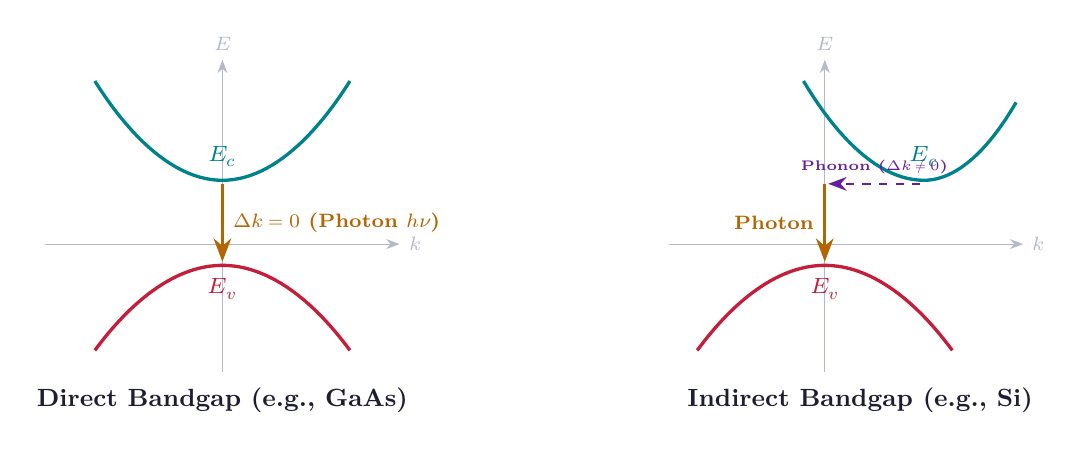
\begin{tikzpicture}[scale=0.9]
  % Direct Bandgap (Left)
  \begin{scope}[xshift=-4.5cm]
    \draw[-Stealth, color=mgframe] (-2.5,0) -- (2.5,0) node[right, font=\scriptsize] {$k$};
    \draw[-Stealth, color=mgframe] (0,-1.8) -- (0,2.6) node[above, font=\scriptsize] {$E$};
    % Conduction Band parabola
    \draw[very thick, color=myteal] (-1.8, 2.3) parabola bend (0, 0.9) (1.8, 2.3);
    \node[above, font=\footnotesize\bfseries\color{myteal}] at (0, 0.95) {$E_c$};
    % Valence Band parabola
    \draw[very thick, color=myred] (-1.8, -1.5) parabola bend (0, -0.3) (1.8, -1.5);
    \node[below, font=\footnotesize\bfseries\color{myred}] at (0, -0.35) {$E_v$};
    % Direct vertical transition
    \draw[-Stealth, very thick, color=myamber] (0, 0.85) -- (0, -0.25) node[midway, right, font=\scriptsize\bfseries\color{myamber}] {$\Delta k = 0$ (Photon $h\nu$)};
    \node[font=\small\bfseries\color{mydark}] at (0, -2.2) {Direct Bandgap (e.g., GaAs)};
  \end{scope}

  % Indirect Bandgap (Right)
  \begin{scope}[xshift=4.0cm]
    \draw[-Stealth, color=mgframe] (-2.2,0) -- (2.8,0) node[right, font=\scriptsize] {$k$};
    \draw[-Stealth, color=mgframe] (0,-1.8) -- (0,2.6) node[above, font=\scriptsize] {$E$};
    % Conduction Band parabola (shifted minimum)
    \draw[very thick, color=myteal] (-0.3, 2.3) parabola bend (1.4, 0.9) (2.7, 2.0);
    \node[above, font=\footnotesize\bfseries\color{myteal}] at (1.4, 0.95) {$E_c$};
    % Valence Band parabola (centered at k=0)
    \draw[very thick, color=myred] (-1.8, -1.5) parabola bend (0, -0.3) (1.8, -1.5);
    \node[below, font=\footnotesize\bfseries\color{myred}] at (0, -0.35) {$E_v$};
    % Two-step transition (phonon + photon)
    \draw[-Stealth, thick, dashed, color=mypurple] (1.35, 0.85) -- (0.05, 0.85) node[midway, above, font=\tiny\bfseries\color{mypurple}] {Phonon ($\Delta k \neq 0$)};
    \draw[-Stealth, very thick, color=myamber] (0, 0.85) -- (0, -0.25) node[midway, left, font=\scriptsize\bfseries\color{myamber}] {Photon};
    \node[font=\small\bfseries\color{mydark}] at (0.5, -2.2) {Indirect Bandgap (e.g., Si)};
  \end{scope}
\end{tikzpicture}
\end{tcolorbox}

% ===============================================================================
\section{Classification: Metals, Semiconductors, and Insulators}
% ===============================================================================

Solids are classified into three categories based on the magnitude of their forbidden energy gap ($E_g$) and their room-temperature electrical conductivity:

\par\vspace{6pt}\noindent
\begingroup
\setlength{\tabcolsep}{3.5pt}
\setlength{\extrarowheight}{3pt}
\renewcommand{\arraystretch}{1.35}
\begin{tabularx}{\linewidth}{|B{2.4cm}|Y|Y|Y|}
\hline
\textbf{Parameter} & \textbf{Insulator} & \textbf{Semiconductor} & \textbf{Metal (Conductor)} \\
\hline
Forbidden Gap ($E_g$) & Very large ($E_g > 3\,\text{eV}$ to $6\,\text{eV}$) & Moderate ($0.6\,\text{eV} \le E_g \le 2.0\,\text{eV}$) & Zero ($E_g = 0\,\text{eV}$, bands overlap) \\
\hline
Conduction Band at $0\,\text{K}$ & Completely empty & Completely empty & Partially filled or overlaps VB \\
\hline
Conductivity ($\sigma$) & Extremely low ($< 10^{-10}\,\text{S/cm}$) & Intermediate ($10^{-6}$ to $10^{2}\,\text{S/cm}$) & Extremely high ($10^{4}$ to $10^{6}\,\text{S/cm}$) \\
\hline
Temperature Coefficient of Resistance & Negative ($\text{NTC}$): Resistance decreases as $T$ increases & Negative ($\text{NTC}$): $R$ decreases exponentially as $T$ rises & Positive ($\text{PTC}$): Resistance increases due to phonon scattering \\
\hline
Typical Materials & Diamond ($5.5\,\text{eV}$), $\text{SiO}_2$ ($9\,\text{eV}$) & $\text{Si}$ ($1.12\,\text{eV}$), $\text{Ge}$ ($0.66\,\text{eV}$), $\text{GaAs}$ & Copper ($\text{Cu}$), Aluminum ($\text{Al}$), Gold \\
\hline
\end{tabularx}
\endgroup

\subsection{Temperature Dependence of Bandgap Energy}
The bandgap of a semiconductor decreases slightly as temperature increases due to thermal lattice expansion and increased electron-phonon interaction. Varshni's empirical formula models this variation:

\begin{equation}
  E_g(T) = E_g(0) - \frac{\alpha T^2}{T + \beta}
\end{equation}

For Silicon: $E_g(0) = 1.17\,\text{eV}$, $\alpha = 4.73 \times 10^{-4}\,\text{eV/K}$, $\beta = 636\,\text{K}$. At $300\,\text{K}$, $E_g \approx 1.12\,\text{eV}$.

% ===============================================================================
\section{Fermi Level and Carrier Statistics}
% ===============================================================================

\subsection{Fermi-Dirac Distribution Function}
Electrons are fermions (spin-$1/2$ particles) subject to the Pauli exclusion principle. The probability $f(E)$ that an available quantum energy state $E$ is occupied by an electron at thermodynamic equilibrium temperature $T$ is governed by the \textbf{Fermi-Dirac distribution}:

\begin{equation}
  f(E) = \frac{1}{1 + \exp\left(\displaystyle\frac{E - E_F}{k T}\right)}
\end{equation}

where $k = 8.617 \times 10^{-5}\,\text{eV/K} = 1.38 \times 10^{-23}\,\text{J/K}$ is Boltzmann's constant, and $E_F$ is the \textbf{Fermi energy level}.

\begin{tcolorbox}[defbox, title={\textbf{Physical Meaning and Properties of Fermi Level $E_F$}}]
\begin{itemize}[leftmargin=*, itemsep=3pt, topsep=0pt]
  \item At absolute zero ($T = 0\,\text{K}$):
    \begin{equation}
      f(E) = 
      \begin{cases} 
        1, & E < E_F \quad \text{(all states below $E_F$ are completely filled)} \\ 
        0, & E > E_F \quad \text{(all states above $E_F$ are completely empty)} 
      \end{cases}
    \end{equation}
    $E_F$ is the highest filled energy level at absolute zero temperature.
  \item At any finite temperature ($T > 0\,\text{K}$):
    When $E = E_F$, the exponential argument vanishes:
    \begin{equation}
      f(E_F) = \frac{1}{1 + e^0} = \frac{1}{2} = 0.5
    \end{equation}
    The Fermi level is the energy state having a $50\%$ probability of being occupied by an electron.
  \item The probability of a state at $E$ being empty (occupied by a hole) is:
    \begin{equation}
      1 - f(E) = \frac{1}{1 + \exp\left(\displaystyle\frac{E_F - E}{k T}\right)}
    \end{equation}
\end{itemize}
\end{tcolorbox}

\begin{tcolorbox}[tikzbox, title={Fermi-Dirac Distribution at Different Temperatures}]
\centering
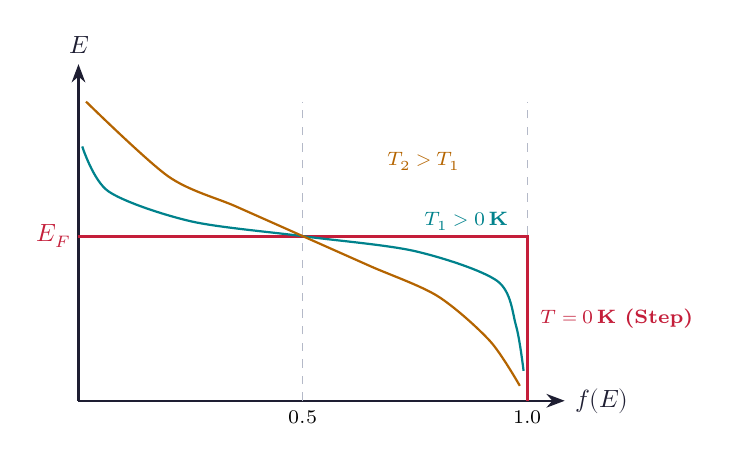
\begin{tikzpicture}[scale=0.95]
  \draw[-Stealth, thick, color=mydark] (0,0) -- (6.5,0) node[right, font=\small] {$f(E)$};
  \draw[-Stealth, thick, color=mydark] (0,0) -- (0,4.5) node[above, font=\small] {$E$};

  % Coordinates
  \coordinate (O) at (0,0);
  \coordinate (fhalf) at (3.0, 2.2);
  \coordinate (EF) at (0, 2.2);
  \coordinate (f1) at (6.0, 0);

  % Axis ticks and labels
  \draw[dashed, color=mgframe] (3.0, 0) -- (3.0, 4.0);
  \node[below, font=\scriptsize] at (3.0, 0) {$0.5$};
  \draw[dashed, color=mgframe] (6.0, 0) -- (6.0, 4.0);
  \node[below, font=\scriptsize] at (6.0, 0) {$1.0$};
  \node[left, font=\small\bfseries\color{myred}] at (0, 2.2) {$E_F$};

  % T = 0 K step function
  \draw[very thick, color=myred] (6.0, 0) -- (6.0, 2.2) -- (0, 2.2);
  \node[right, font=\scriptsize\bfseries\color{myred}] at (6.05, 1.1) {$T = 0\,\text{K}$ (Step)};

  % T1 > 0 K curve
  \draw[thick, color=myteal, smooth] plot coordinates {
    (5.95, 0.4) (5.85, 1.0) (5.6, 1.6) (4.5, 2.0) (3.0, 2.2) (1.5, 2.4) (0.4, 2.8) (0.05, 3.4)
  };
  \node[right, font=\scriptsize\bfseries\color{myteal}] at (4.5, 2.4) {$T_1 > 0\,\text{K}$};

  % T2 > T1 curve
  \draw[thick, color=myamber, smooth] plot coordinates {
    (5.9, 0.2) (5.5, 0.8) (4.8, 1.4) (3.9, 1.8) (3.0, 2.2) (2.1, 2.6) (1.2, 3.0) (0.1, 4.0)
  };
  \node[right, font=\scriptsize\bfseries\color{myamber}] at (4.0, 3.2) {$T_2 > T_1$};
\end{tikzpicture}
\end{tcolorbox}

% ===============================================================================
\section{Intrinsic and Extrinsic Semiconductors}
% ===============================================================================

\subsection{Intrinsic Semiconductors and Intrinsic Carrier Concentration}
An \textbf{intrinsic semiconductor} is a chemically pure semiconductor crystal containing no significant impurities or structural lattice defects.

\begin{itemize}[leftmargin=*, itemsep=3pt]
  \item Free carriers are generated purely by thermal breakage of covalent bonds.
  \item Every electron elevated to the conduction band leaves behind exactly one vacant state (hole) in the valence band:
  \begin{equation}
    n = p = n_i
  \end{equation}
  where $n$ is electron concentration ($\text{cm}^{-3}$), $p$ is hole concentration ($\text{cm}^{-3}$), and $n_i$ is the \textbf{intrinsic carrier concentration}.
  \item For Silicon at $300\,\text{K}$, $n_i \approx 1.5 \times 10^{10}\,\text{cm}^{-3}$. For Germanium, $n_i \approx 2.4 \times 10^{13}\,\text{cm}^{-3}$. For GaAs, $n_i \approx 1.8 \times 10^6\,\text{cm}^{-3}$.
\end{itemize}

\subsection{Effective Density of States and Equilibrium Carrier Concentrations}
Integrating the product of the density of available quantum states $g(E)$ and the Fermi-Dirac distribution $f(E)$ under the Maxwell-Boltzmann approximation ($E - E_F \gg 3kT$) yields:

\begin{tcolorbox}[formulabox, title={\textbf{Equilibrium Carrier Concentrations and Effective Densities of States}}]
\begin{align}
  n_0 &= N_c \exp\left(-\frac{E_c - E_F}{k T}\right) \\
  p_0 &= N_v \exp\left(-\frac{E_F - E_v}{k T}\right)
\end{align}
where $N_c$ and $N_v$ are the \textbf{effective densities of states} in the conduction and valence bands:
\begin{equation}
  N_c = 2\left(\frac{2\pi m_e^* k T}{h^2}\right)^{3/2}, \qquad N_v = 2\left(\frac{2\pi m_h^* k T}{h^2}\right)^{3/2}
\end{equation}
where $m_e^*$ and $m_h^*$ are the density-of-states effective masses for electrons and holes. For Silicon at $300\,\text{K}$, $N_c \approx 2.8 \times 10^{19}\,\text{cm}^{-3}$ and $N_v \approx 1.04 \times 10^{19}\,\text{cm}^{-3}$.
\end{tcolorbox}

\subsection{The Law of Mass Action}
Multiplying the equilibrium electron concentration $n_0$ and hole concentration $p_0$:

\begin{equation}
  n_0 p_0 = N_c N_v \exp\left(-\frac{E_c - E_F + E_F - E_v}{k T}\right) = N_c N_v \exp\left(-\frac{E_g}{k T}\right)
\end{equation}

Because the product is completely independent of the Fermi level $E_F$ and doping concentrations:

\begin{tcolorbox}[formulabox, title={\textbf{Law of Mass Action}}]
Under thermal equilibrium conditions, for any semiconductor (intrinsic or extrinsic):
\begin{equation}
  n_0 p_0 = n_i^2 = N_c N_v \exp\left(-\frac{E_g}{k T}\right)
\end{equation}
The intrinsic carrier concentration depends exponentially on temperature and bandgap:
\begin{equation}
  n_i = \sqrt{N_c N_v}\,\exp\left(-\frac{E_g}{2 k T}\right) \propto T^{3/2} \exp\left(-\frac{E_g}{2 k T}\right)
\end{equation}
\end{tcolorbox}

\subsection{Position of the Intrinsic Fermi Level (\texorpdfstring{$E_i$}{Ei})}
In an intrinsic semiconductor, $n_0 = p_0 = n_i$. Equating $n_0$ and $p_0$:

\begin{align*}
  N_c \exp\left(-\frac{E_c - E_i}{k T}\right) &= N_v \exp\left(-\frac{E_i - E_v}{k T}\right) \\
  \exp\left(\frac{2E_i - (E_c + E_v)}{k T}\right) &= \frac{N_v}{N_c} = \left(\frac{m_h^*}{m_e^*}\right)^{3/2}
\end{align*}

Solving for $E_i$:
\begin{equation}
  E_i = \frac{E_c + E_v}{2} + \frac{3}{4} k T \ln\left(\frac{m_h^*}{m_e^*}\right)
\end{equation}

\textbf{Key Takeaway:} At $T = 0\,\text{K}$, or if $m_e^* = m_h^*$, $E_i$ lies precisely at the midgap: $E_{\text{midgap}} = (E_c + E_v)/2$. Because $m_h^* > m_e^*$ in Silicon, $E_i$ lies slightly above midgap by a few millielectronvolts at $300\,\text{K}$.

\subsection{Extrinsic Semiconductors: n-type and p-type Doping}
Doping is the intentional introduction of specific trace impurity atoms into an intrinsic semiconductor to selectively increase either electron or hole concentration.

\begin{itemize}[leftmargin=*, itemsep=3.5pt]
  \item \textbf{n-type Doping (Donor Impurities):} Pentavalent atoms (Group V: Phosphorus $\text{P}$, Arsenic $\text{As}$, Antimony $\text{Sb}$) replace Silicon atoms. Four valence electrons form covalent bonds, while the fifth weakly bound electron occupies a discrete energy level $E_d$ located very close to the conduction band ($E_c - E_d \approx 0.045\,\text{eV}$ in $\text{Si}$). At room temperature, all donor atoms ionize:
  \begin{equation}
    n_0 \approx N_D, \qquad p_0 = \frac{n_i^2}{N_D} \ll n_0
  \end{equation}
  The Fermi level shifts upward toward the conduction band:
  \begin{equation}
    E_F - E_i = k T \ln\left(\frac{N_D}{n_i}\right) \implies E_c - E_F = k T \ln\left(\frac{N_c}{N_D}\right)
  \end{equation}

  \item \textbf{p-type Doping (Acceptor Impurities):} Trivalent atoms (Group III: Boron $\text{B}$, Gallium $\text{Ga}$, Indium $\text{In}$) replace Silicon atoms. Three valence electrons form bonds, leaving an empty bond that readily accepts an electron from the valence band, creating a mobile hole. The acceptor energy level $E_a$ lies just above the valence band ($E_a - E_v \approx 0.045\,\text{eV}$ in $\text{Si}$). At room temperature:
  \begin{equation}
    p_0 \approx N_A, \qquad n_0 = \frac{n_i^2}{N_A} \ll p_0
  \end{equation}
  The Fermi level shifts downward toward the valence band:
  \begin{equation}
    E_i - E_F = k T \ln\left(\frac{N_A}{n_i}\right) \implies E_F - E_v = k T \ln\left(\frac{N_v}{N_A}\right)
  \end{equation}
\end{itemize}

\begin{tcolorbox}[tikzbox, title={Energy Band Diagrams for Intrinsic, n-type, and p-type Semiconductors}]
\centering
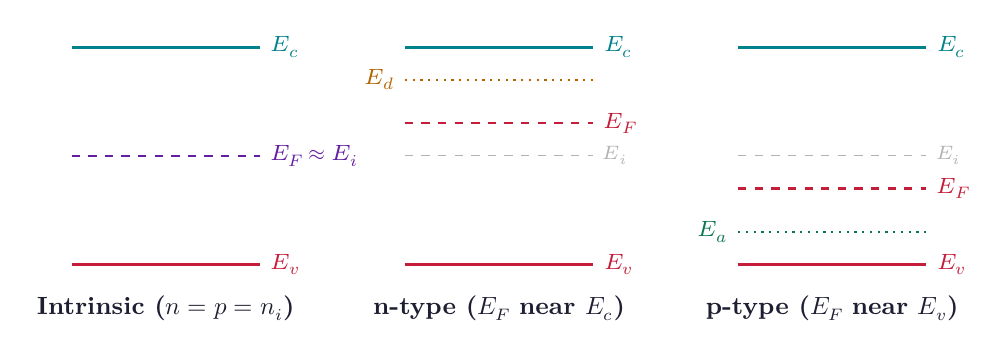
\begin{tikzpicture}[scale=0.92]
  % Intrinsic (Left)
  \begin{scope}[xshift=-4.6cm]
    \draw[very thick, color=myteal] (0, 3.3) -- (2.6, 3.3) node[right, font=\footnotesize\bfseries\color{myteal}] {$E_c$};
    \draw[dashed, thick, color=mypurple] (0, 1.8) -- (2.6, 1.8) node[right, font=\footnotesize\bfseries\color{mypurple}] {$E_F \approx E_i$};
    \draw[very thick, color=myred] (0, 0.3) -- (2.6, 0.3) node[right, font=\footnotesize\bfseries\color{myred}] {$E_v$};
    \node[font=\small\bfseries\color{mydark}] at (1.3, -0.3) {Intrinsic ($n=p=n_i$)};
  \end{scope}

  % n-type (Center)
  \begin{scope}[xshift=0cm]
    \draw[very thick, color=myteal] (0, 3.3) -- (2.6, 3.3) node[right, font=\footnotesize\bfseries\color{myteal}] {$E_c$};
    \draw[dotted, thick, color=myamber] (0, 2.85) node[left, font=\footnotesize\bfseries\color{myamber}] {$E_d$} -- (2.6, 2.85);
    \draw[dashed, thick, color=myred] (0, 2.25) -- (2.6, 2.25) node[right, font=\footnotesize\bfseries\color{myred}] {$E_F$};
    \draw[dashed, thin, color=gray!60] (0, 1.8) -- (2.6, 1.8) node[right, font=\scriptsize\color{gray}] {$E_i$};
    \draw[very thick, color=myred] (0, 0.3) -- (2.6, 0.3) node[right, font=\footnotesize\bfseries\color{myred}] {$E_v$};
    \node[font=\small\bfseries\color{mydark}] at (1.3, -0.3) {n-type ($E_F$ near $E_c$)};
  \end{scope}

  % p-type (Right)
  \begin{scope}[xshift=4.6cm]
    \draw[very thick, color=myteal] (0, 3.3) -- (2.6, 3.3) node[right, font=\footnotesize\bfseries\color{myteal}] {$E_c$};
    \draw[dashed, thin, color=gray!60] (0, 1.8) -- (2.6, 1.8) node[right, font=\scriptsize\color{gray}] {$E_i$};
    \draw[dashed, thick, color=myred] (0, 1.35) -- (2.6, 1.35) node[right, font=\footnotesize\bfseries\color{myred}] {$E_F$};
    \draw[dotted, thick, color=mygreen] (0, 0.75) node[left, font=\footnotesize\bfseries\color{mygreen}] {$E_a$} -- (2.6, 0.75);
    \draw[very thick, color=myred] (0, 0.3) -- (2.6, 0.3) node[right, font=\footnotesize\bfseries\color{myred}] {$E_v$};
    \node[font=\small\bfseries\color{mydark}] at (1.3, -0.3) {p-type ($E_F$ near $E_v$)};
  \end{scope}
\end{tikzpicture}
\end{tcolorbox}

\subsection{Temperature Dependence of Extrinsic Carrier Concentration}
In an n-type semiconductor ($N_D \gg n_i$), electron concentration varies across three distinct temperature regimes:

\begin{enumerate}[label=\arabic*., leftmargin=*]
  \item \textbf{Ionization (Freeze-out) Regime ($T < 100\,\text{K}$):} Thermal energy is insufficient to ionize all donor electrons. As temperature rises, electrons transition from $E_d$ to $E_c$. Carrier concentration increases rapidly: $n_0 \propto \exp(-\Delta E_d / 2kT)$.
  \item \textbf{Extrinsic (Exhaustion / Saturation) Regime ($100\,\text{K} \le T \le 450\,\text{K}$):} All donor impurities are fully ionized, while intrinsic generation across $E_g$ remains negligible ($n_i \ll N_D$). Carrier concentration remains flat and constant: $n_0 \approx N_D$. This is the standard operational regime for electronic devices.
  \item \textbf{Intrinsic Regime ($T > 450\,\text{K}$):} Thermally generated intrinsic carriers across the bandgap exceed the donor concentration ($n_i \gg N_D$). The semiconductor loses its extrinsic properties and behaves as an intrinsic material ($n_0 \approx n_i \propto T^{3/2} e^{-E_g/2kT}$).
\end{enumerate}

% ===============================================================================
\section{Carrier Transport: Drift and Diffusion}
% ===============================================================================

Charge carriers in semiconductors move under the influence of two primary driving forces: electric fields (\textbf{drift}) and carrier concentration gradients (\textbf{diffusion}).

\subsection{Carrier Drift and Mobility}
When an electric field $\mathcal{E}$ is applied across a semiconductor, electrons and holes accelerate until they collide with the vibrating lattice atoms (phonons) or ionized impurity atoms. The net average velocity acquired between collisions is the \textbf{drift velocity} ($v_d$):

\begin{equation}
  v_{d,n} = -\mu_n \mathcal{E}, \qquad v_{d,p} = \mu_p \mathcal{E}
\end{equation}

where $\mu_n$ and $\mu_p$ are the electron and hole \textbf{carrier mobilities} ($\text{cm}^2/\text{V}\cdot\text{s}$):

\begin{equation}
  \mu = \frac{q \tau_c}{m^*}
\end{equation}

where $\tau_c$ is the mean free collision time, and $m^*$ is the conductivity effective mass. Because $m_e^* < m_h^*$ in Silicon, $\mu_n \approx 1350\,\text{cm}^2/\text{V}\cdot\text{s}$ is significantly higher than $\mu_p \approx 480\,\text{cm}^2/\text{V}\cdot\text{s}$.

\subsubsection{Scattering Mechanisms and Temperature Dependence}
By \textbf{Matthiessen's Rule}, the total effective mobility $\mu$ is limited by the reciprocal sum of independent scattering processes:

\begin{equation}
  \frac{1}{\mu} = \frac{1}{\mu_{\text{lattice}}} + \frac{1}{\mu_{\text{impurity}}}
\end{equation}

\begin{itemize}[leftmargin=*, itemsep=3pt]
  \item \textbf{Lattice (Acoustic Phonon) Scattering:} Thermal vibrations of lattice atoms scatter carriers. As temperature increases, lattice vibrations intensify: $\mu_{\text{lattice}} \propto T^{-3/2}$.
  \item \textbf{Ionized Impurity Scattering:} Electrostatic Coulomb deflection of carriers as they travel past ionized donor ($N_D^+$) or acceptor ($N_A^-$) impurities. At higher temperatures, thermal velocity increases, carriers spend less time near impurity ions, and scattering diminishes: $\mu_{\text{impurity}} \propto T^{3/2} / N_I$.
\end{itemize}

\subsection{Drift Current Density and Conductivity}
The current density due to drift of electrons and holes under electric field $\mathcal{E}$ is:

\begin{equation}
  J_{\text{drift}} = J_{n,\text{drift}} + J_{p,\text{drift}} = q n \mu_n \mathcal{E} + q p \mu_p \mathcal{E} = \sigma \mathcal{E}
\end{equation}

where the \textbf{electrical conductivity} $\sigma$ and resistivity $\rho$ are:

\begin{tcolorbox}[formulabox, title={\textbf{Conductivity and Resistivity}}]
\begin{align}
  \sigma &= q (n \mu_n + p \mu_p) \quad (\text{S/cm}) \\
  \rho &= \frac{1}{\sigma} = \frac{1}{q (n \mu_n + p \mu_p)} \quad (\Omega\cdot\text{cm})
\end{align}
For an n-type semiconductor ($n \approx N_D \gg p$): $\sigma \approx q N_D \mu_n$.
\end{tcolorbox}

\subsection{Carrier Diffusion}
Carrier diffusion is the net movement of charge carriers from a region of higher concentration to a region of lower concentration due to random thermal Brownian motion. By Fick's first law of diffusion:

\begin{tcolorbox}[formulabox, title={\textbf{Diffusion Current Densities}}]
\begin{align}
  J_{n,\text{diff}} &= +q D_n \frac{dn}{dx} \\
  J_{p,\text{diff}} &= -q D_p \frac{dp}{dx}
\end{align}
where $D_n$ and $D_p$ are the \textbf{diffusion coefficients} ($\text{cm}^2/\text{s}$). The negative sign in $J_{p,\text{diff}}$ arises because holes diffuse down the concentration gradient ($\nabla p < 0$), carrying positive charge in the direction of diffusion. Electrons carry negative charge, producing a positive sign.
\end{tcolorbox}

\subsection{Total Current Density}
Combining drift and diffusion components yields the complete one-dimensional current equations:

\begin{equation}
  J_n = J_{n,\text{drift}} + J_{n,\text{diff}} = q n \mu_n \mathcal{E} + q D_n \frac{dn}{dx}
\end{equation}
\begin{equation}
  J_p = J_{p,\text{drift}} + J_{p,\text{diff}} = q p \mu_p \mathcal{E} - q D_p \frac{dp}{dx}
\end{equation}
\begin{equation}
  J_{\text{total}} = J_n + J_p
\end{equation}

\subsection{The Einstein Relation}
Under thermodynamic equilibrium, no external current can flow ($J_n = 0, J_p = 0$). Setting $J_p = 0$ in a non-uniformly doped semiconductor where a built-in internal electric field balances carrier diffusion:

\begin{align*}
  q p \mu_p \mathcal{E} &= q D_p \frac{dp}{dx} \\
  \mathcal{E} &= \frac{D_p}{\mu_p} \frac{1}{p} \frac{dp}{dx}
\end{align*}

Using the electrostatic potential $\mathcal{E} = -\frac{dV}{dx}$ and Boltzmann relationship $p(x) = n_i \exp\left(\frac{E_i - E_F}{kT}\right) = n_i \exp\left(-\frac{qV}{kT}\right)$, we find $\frac{1}{p}\frac{dp}{dx} = -\frac{q}{kT}\frac{dV}{dx} = \frac{q}{kT}\mathcal{E}$. Substituting yields:

\begin{tcolorbox}[formulabox, title={\textbf{Einstein Relation}}]
\begin{equation}
  \frac{D_n}{\mu_n} = \frac{D_p}{\mu_p} = \frac{k T}{q} = V_T
\end{equation}
where $V_T = \frac{kT}{q} \approx 25.9\,\text{mV}$ at $T = 300\,\text{K}$ is the \textbf{thermal voltage}.
\end{tcolorbox}

% ===============================================================================
\section{Generation, Recombination, and Minority Carrier Injection}
% ===============================================================================

\subsection{Carrier Generation and Recombination Mechanisms}
\begin{itemize}[leftmargin=*, itemsep=3pt]
  \item \textbf{Generation ($G$):} The process whereby electron-hole pairs are created. Mechanisms include thermal generation ($G_{\text{th}}$) and optical absorption ($G_L$).
  \item \textbf{Recombination ($R$):} The process whereby an electron drops into a vacant hole state, annihilating both carriers and releasing energy.
\end{itemize}

The three principal physical mechanisms of recombination are:
\begin{enumerate}[label=\arabic*., leftmargin=*]
  \item \textbf{Direct Band-to-Band Recombination:} An electron transitions directly from the CB to VB, emitting a photon. Dominates in direct bandgap materials ($\text{GaAs}$). Recombination rate $R \propto n \cdot p$.
  \item \textbf{Shockley-Read-Hall (SRH) Recombination:} Mediated by deep localized energy states or ``traps'' located near the center of the bandgap created by crystal defects or metallic impurities (Gold, Platinum). Dominates in indirect bandgap semiconductors ($\text{Si}, \text{Ge}$).
  \item \textbf{Auger Recombination:} The energy released when an electron recombines with a hole is transferred to a third carrier (electron or hole), kicking it higher into its band. Important under very high injection levels and heavily doped regions.
\end{enumerate}

\subsection{Excess Carriers and Low-Level Injection}
When excess carriers are introduced into a semiconductor (via illumination or forward-biased p-n junction injection):
\begin{equation}
  n(t) = n_0 + \Delta n(t), \qquad p(t) = p_0 + \Delta p(t)
\end{equation}
where $n_0, p_0$ are equilibrium concentrations, and $\Delta n, \Delta p$ are excess carrier concentrations. In non-breakdown conditions, $\Delta n = \Delta p$.

\begin{tcolorbox}[defbox, title={\textbf{Low-Level Injection Condition}}]
Low-level injection occurs when the excess carrier density is much smaller than the thermal equilibrium majority carrier density:
\begin{itemize}[leftmargin=*, itemsep=2pt, topsep=0pt]
  \item For n-type: $\Delta p = \Delta n \ll n_0 \implies n \approx n_0$, but $p = p_0 + \Delta p \gg p_0$.
  \item For p-type: $\Delta n = \Delta p \ll p_0 \implies p \approx p_0$, but $n = n_0 + \Delta n \gg n_0$.
\end{itemize}
Under low-level injection, majority carrier concentration remains virtually unchanged, but minority carrier concentration changes by orders of magnitude.
\end{tcolorbox}

\subsection{Minority Carrier Lifetime and Diffusion Length}
The net rate of recombination of excess minority holes in an n-type material is proportional to the excess density:
\begin{equation}
  R - G_{\text{th}} = \frac{\Delta p}{\tau_p}
\end{equation}
where $\tau_p$ is the \textbf{minority carrier lifetime}. When excess carrier generation ceases at $t=0$, the excess carriers decay exponentially:
\begin{equation}
  \Delta p(t) = \Delta p(0) \exp\left(-\frac{t}{\tau_p}\right)
\end{equation}

During its lifetime $\tau_p$, an excess carrier diffuses an average distance called the \textbf{minority carrier diffusion length} ($L$):

\begin{tcolorbox}[formulabox, title={\textbf{Diffusion Lengths}}]
\begin{equation}
  L_p = \sqrt{D_p \tau_p}, \qquad L_n = \sqrt{D_n \tau_n}
\end{equation}
\end{tcolorbox}

% ===============================================================================
\section{Poisson's Equation and the Continuity Equation}
% ===============================================================================

\subsection{Poisson's Equation}
Poisson's equation relates the spatial distribution of electrostatic potential $V(x)$ and electric field $\mathcal{E}(x)$ to the net volume charge density $\rho(x)$ using Gauss's law ($\nabla \cdot \vec{\mathcal{E}} = \rho/\epsilon_s$):

\begin{tcolorbox}[formulabox, title={\textbf{Poisson's Equation}}]
\begin{equation}
  \frac{d^2 V}{dx^2} = -\frac{d\mathcal{E}}{dx} = -\frac{\rho(x)}{\epsilon_s} = -\frac{q}{\epsilon_s} \left[ p(x) - n(x) + N_D^+(x) - N_A^-(x) \right]
\end{equation}
where $\epsilon_s = \epsilon_r \epsilon_0$ is the semiconductor permittivity ($\epsilon_s = 11.7 \times 8.854 \times 10^{-14}\,\text{F/cm}$ for Silicon).
\end{tcolorbox}

\subsection{Derivation of the Continuity Equation}
Consider an infinitesimal semiconductor slab of cross-sectional area $A$ extending between $x$ and $x + dx$.

\begin{tcolorbox}[tikzbox, title={Differential Slice for Continuity Equation Derivation}]
\centering
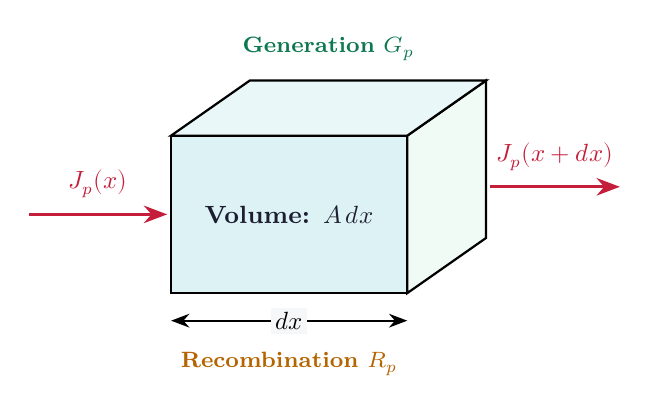
\begin{tikzpicture}[scale=1.0]
  % 3D slab
  \draw[thick, fill=hdrteal] (0,0) rectangle (3.0, 2.0);
  \draw[thick, fill=hdrgreen!40] (3.0,0) -- (4.0, 0.7) -- (4.0, 2.7) -- (3.0, 2.0) -- cycle;
  \draw[thick, fill=hdrteal!60] (0,2.0) -- (1.0, 2.7) -- (4.0, 2.7) -- (3.0, 2.0) -- cycle;

  % Dimension arrows
  \draw[Stealth-Stealth, thick] (0, -0.35) -- (3.0, -0.35) node[midway, fill=mygray, inner sep=1.5pt, font=\small] {$dx$};
  \node[font=\small\bfseries\color{mydark}] at (1.5, 1.0) {Volume: $A\,dx$};

  % Current vectors
  \draw[-Stealth, very thick, color=myred] (-1.8, 1.0) -- (-0.05, 1.0) node[midway, above=2pt, font=\small\bfseries\color{myred}] {$J_p(x)$};
  \draw[-Stealth, very thick, color=myred] (4.05, 1.35) -- (5.7, 1.35) node[midway, above=2pt, font=\small\bfseries\color{myred}] {$J_p(x+dx)$};

  % Generation and Recombination
  \node[font=\footnotesize\bfseries\color{mygreen}] at (2.0, 3.1) {Generation $G_p$};
  \node[font=\footnotesize\bfseries\color{myamber}] at (1.5, -0.9) {Recombination $R_p$};
\end{tikzpicture}
\end{tcolorbox}

The rate of change of total hole charge within the slice must equal the net hole current entering minus exiting, plus generation minus recombination:

\begin{equation}
  \frac{\partial p}{\partial t} A\,dx = \left[ \frac{J_p(x) A}{q} - \frac{J_p(x+dx) A}{q} \right] + (G_p - R_p) A\,dx
\end{equation}

Expanding $J_p(x+dx)$ in a first-order Taylor series:
\begin{equation}
  J_p(x+dx) = J_p(x) + \frac{\partial J_p}{\partial x} dx
\end{equation}

Dividing through by $A\,dx$:

\begin{tcolorbox}[formulabox, title={\textbf{General One-Dimensional Continuity Equations}}]
\begin{align}
  \frac{\partial p}{\partial t} &= -\frac{1}{q} \frac{\partial J_p}{\partial x} + G_p - R_p \quad \text{(Holes)} \\
  \frac{\partial n}{\partial t} &= +\frac{1}{q} \frac{\partial J_n}{\partial x} + G_n - R_n \quad \text{(Electrons)}
\end{align}
\end{tcolorbox}

\subsection{Minority Carrier Diffusion Equation}
Substituting the hole current equation $J_p = q p \mu_p \mathcal{E} - q D_p \frac{\partial p}{\partial x}$ into the continuity equation, setting $R_p - G_{\text{th}} = \frac{\Delta p}{\tau_p}$, and introducing excess optical generation $G_L$:

\begin{equation}
  \frac{\partial (\Delta p)}{\partial t} = D_p \frac{\partial^2 (\Delta p)}{\partial x^2} - \mu_p \mathcal{E} \frac{\partial (\Delta p)}{\partial x} - \mu_p p \frac{\partial \mathcal{E}}{\partial x} + G_L - \frac{\Delta p}{\tau_p}
\end{equation}

For an electric-field-free region ($\mathcal{E} \approx 0$), this simplifies to the celebrated \textbf{Minority Carrier Diffusion Equation}:

\begin{tcolorbox}[formulabox, title={\textbf{Minority Carrier Diffusion Equation (Field-Free Region)}}]
\begin{equation}
  \frac{\partial (\Delta p)}{\partial t} = D_p \frac{\partial^2 (\Delta p)}{\partial x^2} + G_L - \frac{\Delta p}{\tau_p}
\end{equation}
\end{tcolorbox}

\subsubsection{Important Special Case: Steady-State Injection into Semi-Infinite Bar}
Consider a long n-type semiconductor ($x \ge 0$) under steady-state conditions ($\partial/\partial t = 0$), no light ($G_L = 0$), and constant excess hole injection at the surface: $\Delta p(0) = \Delta p_0$. The diffusion equation becomes:

\begin{equation}
  D_p \frac{d^2 (\Delta p)}{dx^2} - \frac{\Delta p}{\tau_p} = 0 \implies \frac{d^2 (\Delta p)}{dx^2} - \frac{\Delta p}{L_p^2} = 0
\end{equation}

Applying boundary conditions:
\begin{itemize}[leftmargin=*, itemsep=2pt]
  \item At $x = 0$: $\Delta p(0) = \Delta p_0$
  \item At $x \to \infty$: $\Delta p(\infty) = 0$
\end{itemize}

The spatial excess carrier profile decays exponentially into the bulk:
\begin{equation}
  \Delta p(x) = \Delta p_0 \exp\left(-\frac{x}{L_p}\right)
\end{equation}
The total injected minority carrier charge per unit area stored in the semiconductor is:
\begin{equation}
  Q_p = q \int_0^\infty \Delta p(x)\,dx = q \Delta p_0 \int_0^\infty e^{-x/L_p}\,dx = q \Delta p_0 L_p
\end{equation}

\newpage
% ===============================================================================
% MANDATORY QUICK REVISION PAGE
% ===============================================================================
\begin{center}
  {\large\bfseries\color{myred} Quick Revision --- Module 1}\\[3pt]
  {\small\color{mydark} Energy Bands \& Current Carriers in Semiconductors $|$ EC301}
\end{center}
\noindent{\color{myred}\rule{\linewidth}{1.2pt}}
\vspace{4pt}

\begin{tcolorbox}[formulabox, title={\textbf{Key Formulas and Metrics at a Glance}}]
\renewcommand{\arraystretch}{1.35}
\begin{tabularx}{\linewidth}{B{5.0cm} X}
Equilibrium Electron Concentration & $n_0 = N_c \exp\left(-\frac{E_c - E_F}{kT}\right)$ \\[4pt]
Equilibrium Hole Concentration & $p_0 = N_v \exp\left(-\frac{E_F - E_v}{kT}\right)$ \\[4pt]
Law of Mass Action & $n_0 p_0 = n_i^2 = N_c N_v \exp\left(-\frac{E_g}{kT}\right)$ \\[4pt]
Intrinsic Fermi Level ($E_i$) & $E_i = \frac{E_c + E_v}{2} + \frac{3}{4} kT \ln\left(\frac{m_h^*}{m_e^*}\right)$ \\[4pt]
Fermi-Dirac Distribution & $f(E) = \frac{1}{1 + \exp\left(\frac{E - E_F}{kT}\right)}$ \\[4pt]
Einstein Relation & $\frac{D_n}{\mu_n} = \frac{D_p}{\mu_p} = \frac{kT}{q} = V_T \approx 25.9\,\text{mV}$ \\[4pt]
Conductivity & $\sigma = q (n\mu_n + p\mu_p)$ \\[4pt]
Total Hole Current Density & $J_p = q p \mu_p \mathcal{E} - q D_p \frac{dp}{dx}$ \\[4pt]
Total Electron Current Density & $J_n = q n \mu_n \mathcal{E} + q D_n \frac{dn}{dx}$ \\[4pt]
Minority Diffusion Length & $L_p = \sqrt{D_p \tau_p}, \quad L_n = \sqrt{D_n \tau_n}$ \\[4pt]
Continuity Equation (Holes) & $\frac{\partial p}{\partial t} = -\frac{1}{q} \frac{\partial J_p}{\partial x} + G_p - R_p$ \\[4pt]
Poisson's Equation & $\frac{d^2 V}{dx^2} = -\frac{q}{\epsilon_s}(p - n + N_D^+ - N_A^-)$ \\[4pt]
\end{tabularx}
\end{tcolorbox}

\begin{tcolorbox}[defbox, title={\textbf{One-Line Definitions}}]
\begin{itemize}[leftmargin=*, itemsep=2pt, topsep=0pt]
  \item \textbf{Covalent Bonding:} Interatomic sharing of valence electron pairs yielding stable octet configurations.
  \item \textbf{Direct Bandgap:} Semiconductor where CB minimum and VB maximum align at the same crystal wavevector ($k=0$).
  \item \textbf{Indirect Bandgap:} Semiconductor where CB minimum is shifted in $k$-space relative to VB maximum, requiring phonon assistance.
  \item \textbf{Fermi Level ($E_F$):} The thermodynamic energy state possessing a $50\%$ probability of occupancy by an electron at $T > 0\,\text{K}$.
  \item \textbf{Intrinsic Semiconductor:} Pure crystalline semiconductor with equal electron and hole concentrations ($n=p=n_i$).
  \item \textbf{Concept of Hole:} Vacant quantum state in the valence band behaving as a mobile positive particle of charge $+q$.
  \item \textbf{Law of Mass Action:} Principle stating that $n_0 p_0 = n_i^2$ is constant at fixed temperature regardless of doping.
  \item \textbf{Carrier Mobility ($\mu$):} Drift velocity per unit applied electric field ($v_d / \mathcal{E}$).
  \item \textbf{Diffusion Length ($L$):} Average distance an injected minority carrier diffuses before recombining.
  \item \textbf{Low-Level Injection:} State where excess injected carrier density is negligible compared to majority carrier concentration.
\end{itemize}
\end{tcolorbox}

\begin{tcolorbox}[exambox, title={\textbf{Frequently Asked / Viva Questions}}]
\begin{enumerate}[topsep=0pt, label=\textbf{Q\arabic*.}, itemsep=5pt]
  \item \Q{Why does Silicon exhibit a negative temperature coefficient of resistance while Copper has a positive one?}
    In semiconductors (Silicon), thermal energy exponentially increases carrier density ($n_i \propto e^{-E_g/2kT}$), which vastly outweighs mobility degradation, making resistance drop ($\text{NTC}$). In metals (Copper), carrier concentration is fixed, and increasing temperature enhances lattice scattering, lowering conductivity ($\text{PTC}$).
  \item \Q{Why is Silicon preferred over Germanium for semiconductor manufacturing?}
    \begin{itemize}[leftmargin=*, itemsep=1pt, topsep=2pt]
      \item Wider bandgap ($1.12\,\text{eV}$ vs $0.66\,\text{eV}$), yielding much lower reverse saturation leakage current ($I_0 \propto n_i^2$).
      \item Higher maximum operating junction temperature ($150^\circ\text{C}$ vs $75^\circ\text{C}$).
      \item Silicon naturally forms a stable, insulating, high-quality native oxide layer ($\text{SiO}_2$), which is critical for planar IC fabrication.
    \end{itemize}
  \item \Q{Why are direct bandgap materials used for LEDs while Silicon is not?}
    In direct bandgap semiconductors ($\text{GaAs}$), electrons transition across the bandgap directly releasing photons without momentum change ($\Delta k = 0$). In Silicon (indirect bandgap), radiative recombination requires a three-particle interaction (electron, hole, phonon), which has extremely low probability; non-radiative thermal dissipation dominates.
  \item \Q{State the Law of Mass Action and its domain of validity.}
    $n_0 p_0 = n_i^2$. It holds strictly under thermal equilibrium in non-degenerate semiconductors. It is invalid under external optical excitation, forward bias injection, or in degenerate semiconductors where $E_F$ enters the bands.
  \item \Q{What is the physical significance of the Einstein Relation?}
    $\frac{D}{\mu} = \frac{kT}{q} = V_T$. It establishes that carrier drift (field-driven transport) and carrier diffusion (thermally driven concentration transport) are fundamentally governed by the same thermal scattering and collision mechanisms.
  \item \Q{Explain the physical meaning of effective mass ($m^*$).}
    Effective mass accounts for the internal periodic potential forces of the crystal lattice on an electron: $m^* = \hbar^2 / \left(\frac{d^2 E}{dk^2}\right)$. It allows Newton's second law ($F = m^* a$) to be applied using only external forces.
  \item \Q{What happens to the Fermi level of an n-type semiconductor as temperature increases to very high values?}
    As temperature increases, intrinsic carrier generation across the bandgap overwhelms donor doping ($n_i \gg N_D$). The semiconductor enters the intrinsic regime, and the Fermi level $E_F$ shifts down from near $E_c$ back toward the intrinsic level $E_i$ (midgap).
  \item \Q{Differentiate between drift and diffusion currents.}
    Drift current is driven by an applied electric field causing directed carrier acceleration. Diffusion current is driven by spatial concentration gradients causing random thermal diffusion from high to low density regions.
  \item \Q{Define minority carrier lifetime and diffusion length.}
    Minority carrier lifetime ($\tau$) is the average time an excess minority carrier survives before recombining. Minority carrier diffusion length ($L = \sqrt{D\tau}$) is the average distance it travels by diffusion during that lifetime.
  \item \Q{What is the significance of the Continuity Equation in semiconductor physics?}
    It enforces the law of conservation of charge carriers across any semiconductor volume element by balancing carrier accumulation against spatial current divergence, net thermal/optical generation, and recombination.
\end{enumerate}
\end{tcolorbox}

\begin{tcolorbox}[tikzbox, title={Comparison of Direct vs. Indirect Bandgap Semiconductors}]
\centering
\renewcommand{\arraystretch}{1.45}
\begin{tabularx}{\linewidth}{|B{3.4cm}|Y|Y|}
\hline
\multicolumn{1}{|c|}{\textbf{Feature}} & \multicolumn{1}{c|}{\textbf{Direct Bandgap}} & \multicolumn{1}{c|}{\textbf{Indirect Bandgap}} \\
\hline
$k$-space Band Alignment & CB minimum and VB maximum occur at identical $k$ ($k=0$) & CB minimum is shifted in $k$-space relative to VB maximum ($k \neq 0$) \\
\hline
Recombination Mechanism & Direct radiative photon emission ($\Delta k = 0$) & Requires simultaneous emission/absorption of a phonon for momentum balance \\
\hline
Radiative Efficiency & Extremely high ($10\%$ to $>50\%$) & Extremely low ($< 0.01\%$, nonradiative dominated) \\
\hline
Carrier Lifetime ($\tau$) & Very short (nanoseconds, $\sim 1\,\text{ns}$ to $10\,\text{ns}$) & Much longer (microseconds, $\sim 1\,\mu\text{s}$ to $1\,\text{ms}$) \\
\hline
Typical Applications & LEDs, Laser Diodes, Photodetectors, High-frequency MMICs & Microprocessors, Memory chips, Power electronic devices \\
\hline
Examples & $\text{GaAs}$, $\text{InP}$, $\text{GaN}$, $\text{InGaAs}$ & $\text{Si}$, $\text{Ge}$, $\text{AlAs}$, $\text{GaP}$ \\
\hline
\end{tabularx}
\end{tcolorbox}

\end{document}
